\documentclass[solutions]{esg8022pset} 
\usepackage{amsmath}
\usepackage{amssymb}
\usepackage{enumerate}
\usepackage{graphicx}
\usepackage{hyperref}
\usepackage{mathtools}
%\usepackage[per-mode=symbol]{siunitx} %If this line is giving you trouble, try replacing per-mode with per
%use inter-unit-separator={}\cdot{} ?
\providecommand{\uvec}[1]{{\hat{\bf{#1}}}}
%\usepackage{pgf,tikz}
%\usetikzlibrary{arrows}
\usepackage{wasysym}
\usepackage{subfig}
\makeatletter
\newcommand{\interitemtext}[1]{%
  \begin{list}{}
   {\itemindent=0mm\labelsep=0mm
   \labelwidth=0mm\leftmargin=0mm
   \addtolength{\leftmargin}{-\@totalleftmargin}}
    \item #1
  \end{list}
}
\makeatother
\renewcommand{\d}{\,d}
\providecommand{\norm}[1]{\lVert#1\rVert}

\AtBeginDocument{%
  % Appologies to any future editor on the inconsistencies in TeX code and the unnecessary braces.  I'm aggregating previously typeset problems, and didn't think it worth my time to improve the quality of TeX code in ways that won't make any difference to the typeset material. -Jason Gross (jgross@mit.edu)
}%
\classname{Physics 8.022} \semester{Spring 2011} 
\problemsetnumber{10}
\date{\today }
\duedate{Wednesday, April 27th, 10 pm}
\readingassignment{}
\problemsettitle{RLC circuits, AC circuits}
\begin{document}
\section{Problem \thesection: Purcell 7.17}
\subsection{Problem}
  In the circuit shown in the diagram the 10-volt battery has negligible
  internal resistance.  The switch $S$ is closed for several seconds, then
  opened.  Make a graph with the potential of point $A$ with respect to
  ground, just before and then for 10 milliseconds after the opening of
  switch $S$.  Show also the variation of the potential at point $B$ in the
  same period of time.

  \begin{center}
    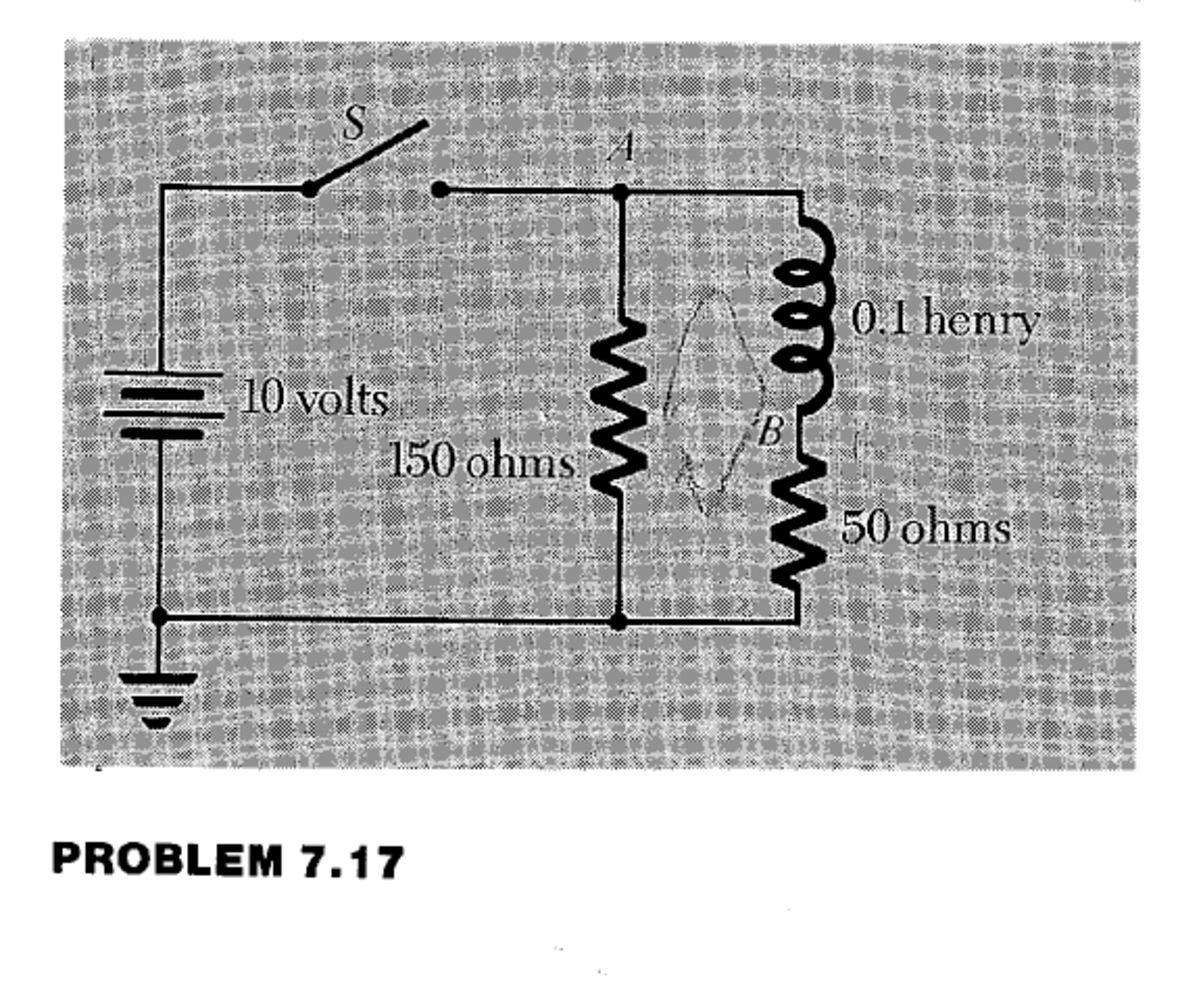
\includegraphics[width = 0.6\textwidth]{figpu717}
  \end{center}

  Extra question --- By grounding this circuit, we make the switch
  safer to operate. Describe why a large spark jumps across the switch
  when it is not grounded, and why the spark does not happen when it is
  grounded.
\subsection{Solution}
  \begin{figure}[H]
    \centering
    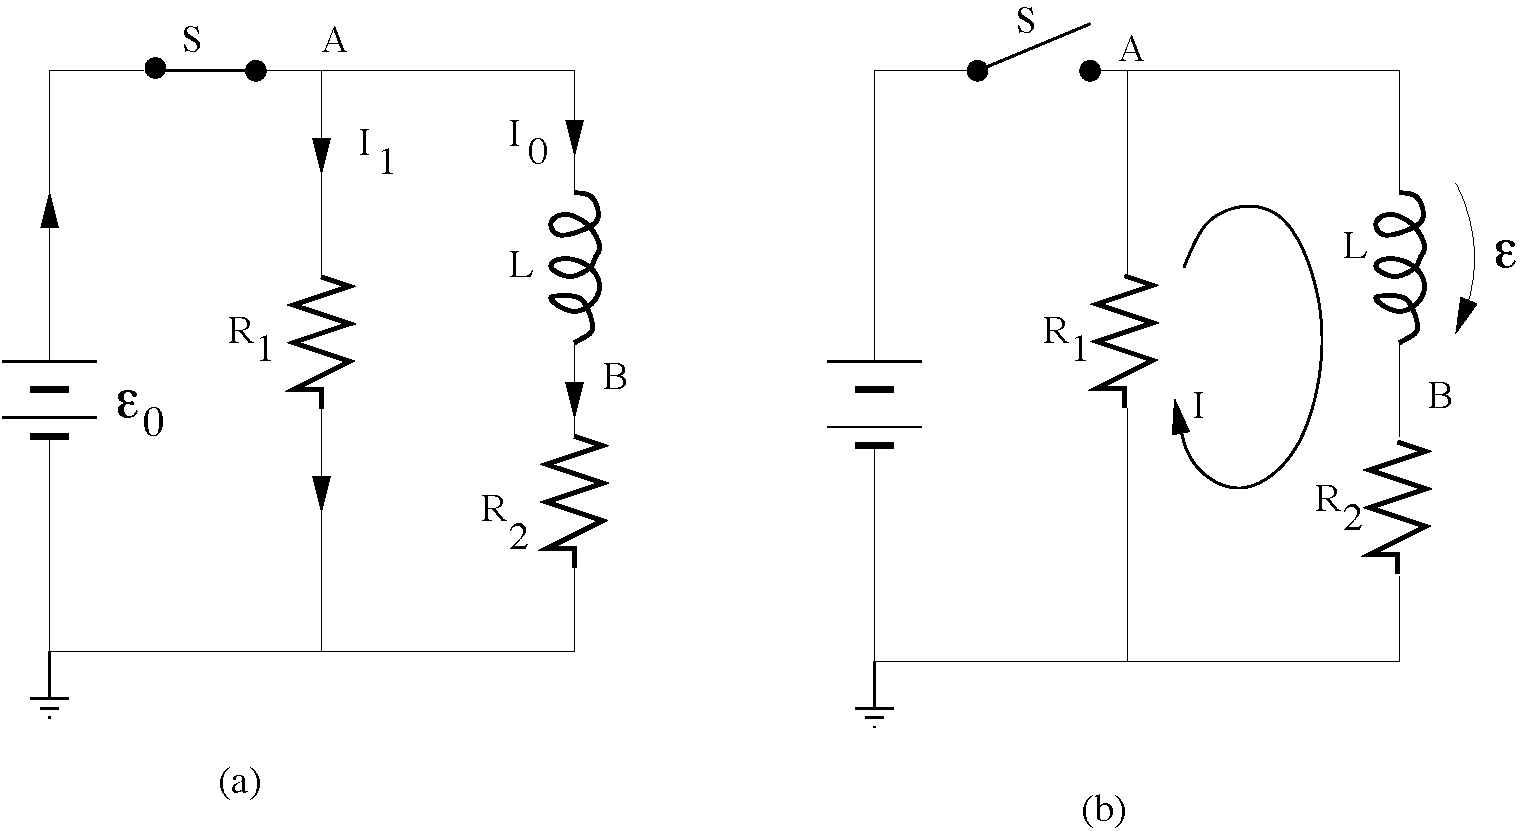
\includegraphics[width = 10cm]{inductance2}
    \caption{LR circuit: (a) steady state when switch S has been closed for a
      long time; (b) the current in LR circuit when switch S is opened.}
    \label{fig:inductance2.eps}
  \end{figure}

  Note: we'll use SI unit in this problem for convenience; and below
  ${\mathcal{E}}_0=10\:\text{volts}$, $R_1=150\:\text{ohms}$, $R_2=50\:\text{ohms}$,
  $L=0.1\:\text{henry}$.\\

  Switch $S$ is closed (see \autoref{fig:inductance2.eps}a) for several
  seconds, which is long enough that the current in the inductor is
  steady; hence the EMF due to the inductor ${\mathcal{E}}=0$.  Right
  right before $S$ is opened, the current on $L$ is $I_0 =
  {\mathcal{E}}_0/R_2 = 0.2\:\text{amp}$.  The potential of point $A$ with
  respect to ground is, for $t<0$, $V_A = {\mathcal{E}}_0 = 10\:\text{volts}$;
  and the potential of point B is, for $t<0$, $V_B=I_0 R_2=
  {\mathcal{E}}_0=10\:\text{volts}$.\\

  After switch S has been opened (Figure \ref{fig:inductance2.eps}b),
  current will decay in the loop containing $L$, $R_2$ and $R_1$, and
  the change in current induces an electromotive force $\mathcal{E}$ on
  the inductor.  Define the positive electromotive force and positive
  current as shown in Figure \ref{fig:inductance2.eps}b; under this
  convention, they satisfy ${\mathcal{E}}=-L\frac{dI}{dt}$.  Apply
  Kirchhoff's rule,
  \begin{equation}
  -{\mathcal{E}}+I(R_1+R_2)=0.
  \end{equation}
  A simple calculation gives an ordinary differential equation for I:
  \begin{equation}\label{eqn3:eom}
  L\frac{dI}{dt}=-(R_1+R_2)I.
  \end{equation}
  The solution of \autoref{eqn3:eom} with initial condition
  $I(t=0)=I_0$ is, for $t>0$,
  \begin{align}
  I(t) & = I_0 e^{-t/\tau},\\
  \text{where}\qquad \tau & = L/(R_1+R_2)=0.5\: \text{milliseconds}.
  \end{align}
  The potentials of point A and point B with respect to ground are, for $t>0$
  \begin{align}
  V_A & = -I(t)R_1=-I_0 R_1 e^{-t/\tau}= -30e^{-t/0.5}\;\text{volts};\\
  V_B & = I(t)R_2=I_0 R_2 e^{-t/\tau}= 10\;e^{-t/0.5}\;\text{volts},
  \end{align}
  where $t$ is in milliseconds.  The plots of potentials Vs. time are
  shown in \autoref{fig:graph22.eps}.


  \begin{figure}[H]
    \centering
    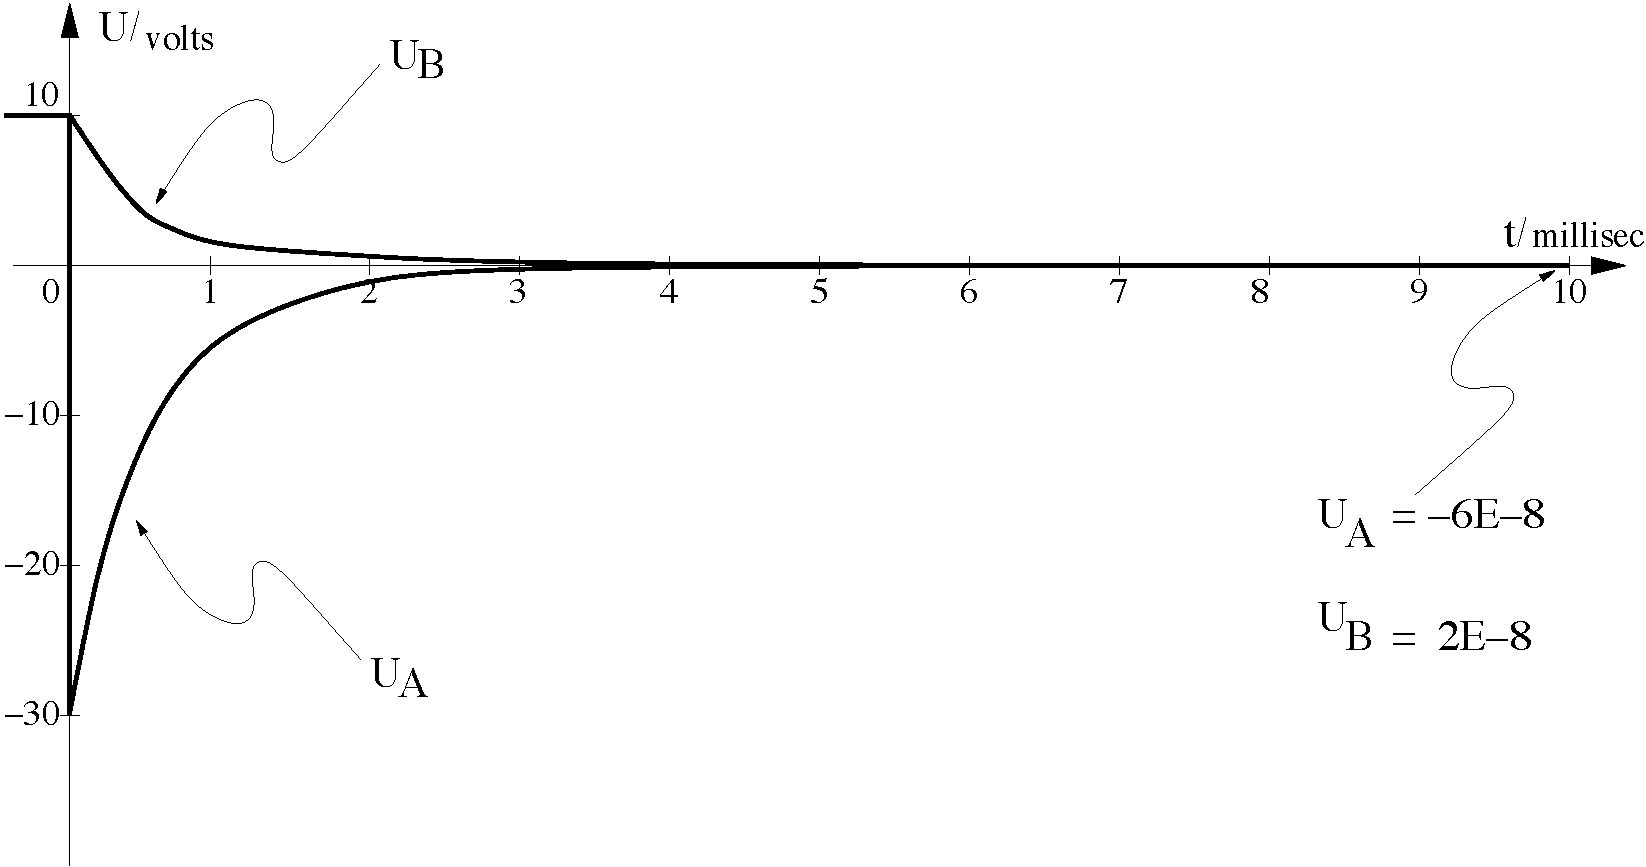
\includegraphics[width = 10cm]{graph22}
    \caption{The exponential decay of the potentials in the LR circuit.
      At $t<0$, both $V_A$ and $V_B$ are at 10 volts; at $t=0$, $V_A$
      abruptly drops to -30 volts, while $V_B$ is continuous.}
    \label{fig:graph22.eps}
  \end{figure}


  Additional question:

  Notice that the current in the 150 Ohm resistor has to abruptly switch
  magnitude and direction at the moment that the switch is opened. If
  the circuit were not grounded, the only way to suddenly change the
  direction of the current would be to ``suck'' the current needed to
  maintain continuity over from the battery -- zap!

  Ground fixes this: we can think of ground as an infinite sink or
  source of charge, and hence of current. By sucking (or dumping) the
  current needed from ground, the current in the 150 Ohm resistor can
  switch directions very rapidly -- there is no need for a big zap
  across the switch.
\section{Problem \thesection: Purcell 8.4}
\subsection{Problem}
  In the resonant circuit shown in the figure below, the dissipative
  element is a resistor $R'$ connected in parallel rather than in series,
  with the $LC$ combination.  Work out the equation analogous to Equation 2
  in Purcell,
  \begin{equation*}
    \frac{d^2V}{dt^2} + \left(\frac{R}{L}\right)\frac{dV}{dt} + \left(\frac{1}{LC}\right)V = 0,
  \end{equation*}
  which applies to this circuit.  Find also the conditions on the solution
  analogous to those that hold in the series $RLC$ circuit.  If a series
  $RLC$ and a parallel $R'LC$ circuit have the same $L$, $C$, and $Q$
  (quality factor), how must $R'$ be related to $R$?

  \begin{center}
    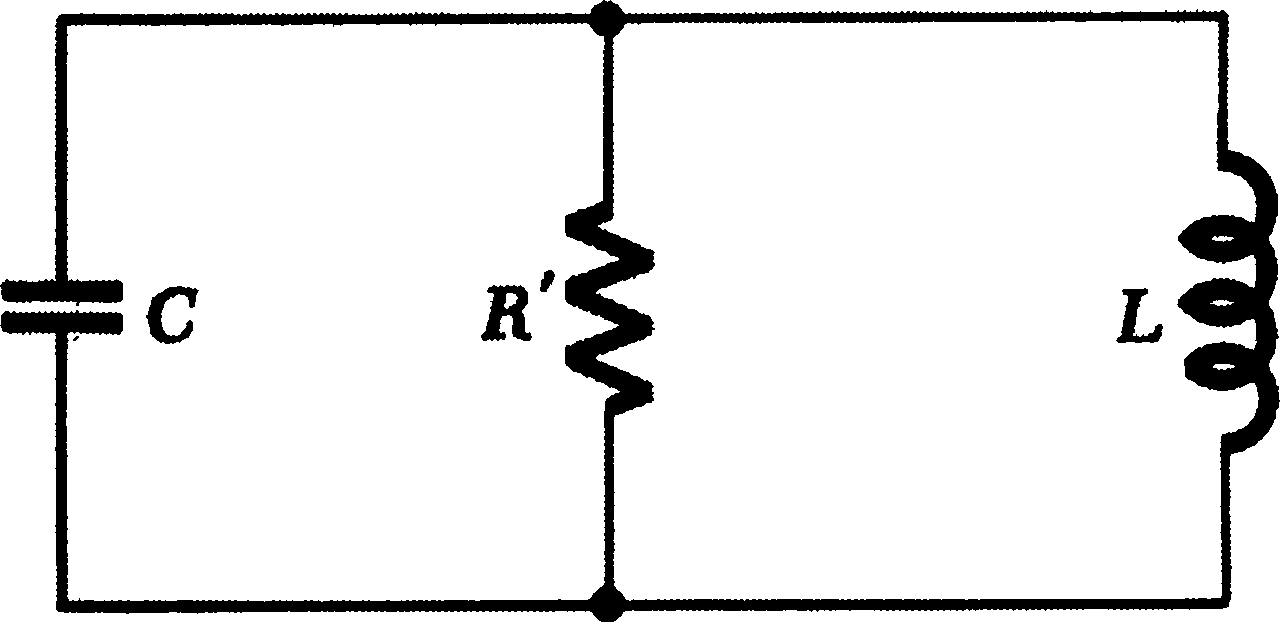
\includegraphics[width = 0.6\textwidth]{figpu804}
  \end{center}
\subsection{Solution}
  \begin{figure}[H]
    \centering
    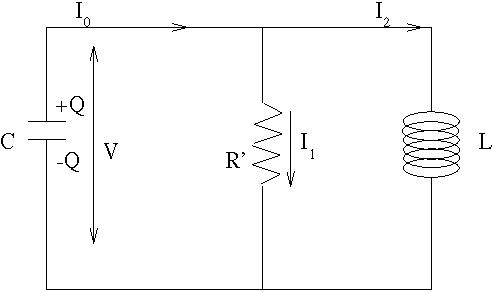
\includegraphics[width = 10cm]{ps8}
    \caption{RLC circuit}
    \label{fig:graph22.eps}
  \end{figure}

  If $V=Q/C$ is the voltage drop across the capacitor, then Kirchoff's
  laws for the left and right-hand loops above give:
  \begin{equation}
  V-I_1R'=0
  \end{equation}

  \begin{equation}
  -L\frac{dI_2}{dt}+I_1R'=0
  \end{equation}

  \begin{equation}
  I_0=I_1+I_2
  \end{equation}

  We also know that $I_0=-dQ/dt$ and that $Q=CV$, so we can write
  \begin{equation}
  I_0=-C\frac{dV}{dt}
  \end{equation}

  The first Kirchoff equation gives us $I_1=V/R'$. The derivative
  $dI_2/dt$ in the second equation can be written:
  \begin{equation}
  \frac{dI_2}{dt}=\frac{d(I_0-I_1)}{dt}=\frac{dI_0}{dt}-\frac{dI_1}{dt}=-C\frac{d^2V}{dt^2}-\frac{1}{R'}\frac{dV}{dt}
  \end{equation}

  Thus we can rewrite the second Kirchoff equation as a differential
  equation for $V$:
  \begin{equation}\label{eqn1:v}
  \frac{d^2V}{dt^2}+\left(\frac{1}{CR'}\right)\frac{dV}{dt}+\left(\frac{1}{LC}\right)V=0
  \end{equation}
  Compare this to the differential equation for $V$ in the case of a
  serial LRC circuit, Purcell, Ch.8, eq.(2).
  \begin{equation}\label{eqn1:v2}
  \frac{d^2V}{dt^2}+\left(\frac{R}{L}\right)\frac{dV}{dt}+\left(\frac{1}{LC}\right)V=0
  \end{equation}
  Thus the solution to \autoref{eqn1:v} can be read off directly
  from the solution to \autoref{eqn1:v2} (i.e. the discussion
  following eq.(2) of Purcell Ch.8) by the substitution
  \begin{align}
  R &\rightarrow & \frac{L}{R'C}\\ \text{and in particular}\qquad
  \alpha=\frac{R}{2L} &\rightarrow & \alpha'=\frac{1}{2R'C}
  \end{align}
  Analogous to the serial RLC, the oscillation frequency is real and hence
  the solution oscillates when $\alpha'<\omega_0=1/\sqrt{LC}$; this
  means we must have
  \begin{equation}
  R'>\frac{1}{2}\sqrt{\frac{L}{C}}
  \end{equation}
  When the parallel and serial circuits have the same $L$, $C$, and quality
  factor $Q$ (not to be confused with the charge on the capacitor), we
  want to find a relation between $R'$ and $R$.  Recall that the quality
  factor for the serial RLC may be written
  \begin{equation}
  Q=\frac{\omega}{2\alpha}=\frac{\sqrt{\omega_0^2-\alpha^2}}{2\alpha}
  \end{equation}
  Thus $Q$ for the parallel RLC
  \begin{equation}
  Q'=\frac{\sqrt{\omega_0^2-\alpha'^2}}{2\alpha'}
  \end{equation}
  Clearly $Q'=Q$ implies that $\alpha'=\alpha$, or $R'=L/RC$.

\section{Problem \thesection: Purcell 8.7}
\subsection{Problem}
  A resonant cavity of the form illustrated is an essential part of many
  microwave oscillators. It can be regarded as a simple $LC$ circuit. The
  inductance is that of a toroid with one turn. Find an expression for the
  resonant frequency of this circuit and show by a sketch the configuration
  of the magnetic and electric fields.
  Hint: the capacitor is composed by the upper and lower disks
  \begin{center}
    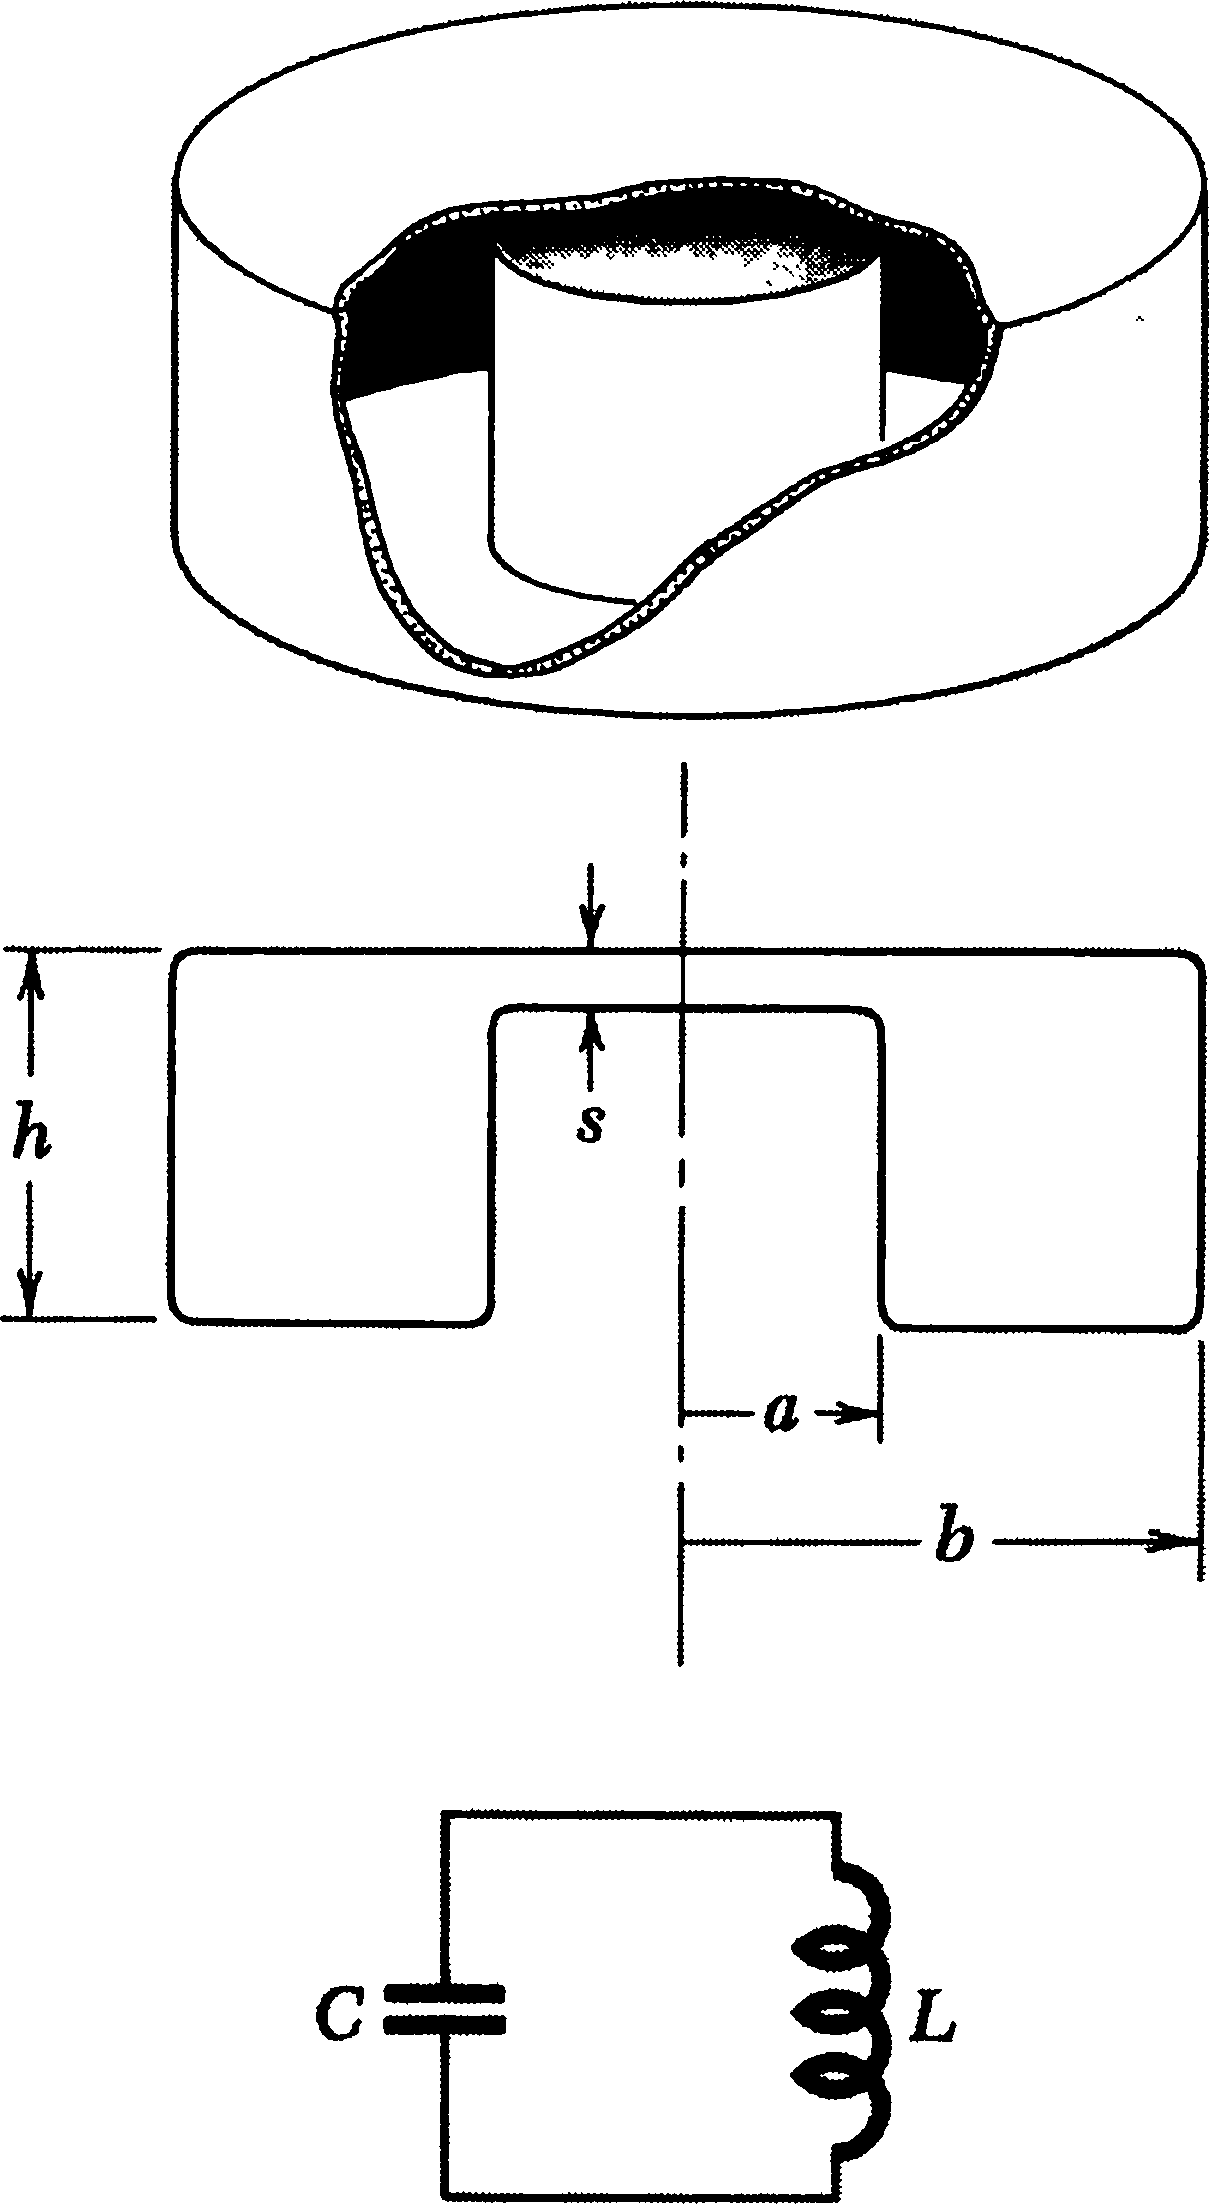
\includegraphics[width = 4cm]{pu807}
  \end{center}
\subsection{Solution}
  The resonant cavity is equivalent to a simple LC circuit.  The
  inductor is a configuration of currents uniformly flowing up and down
  on the surface of the inner conducting cylinder and the outer one.
  The capacitor is a pair of parallel plates of separation $s$ and area
  $A=\pi a^2$.  Quote the result in Problem 8 of pset 8: the inductance
  \emph{per unit length} is
  \[ L/l =\frac{2}{c^2}\ln{(\frac{b}{a})}.\]
  This gives the total inductance
  \[ L= (h-s)\frac{2}{c^2}\ln{(\frac{b}{a})}.\]
  [You could also use Purcell (58) of Chapter 7; you would get $h$ in place of $h-s$, which is good enough
  for small $s$.]

  The capacitor is $C= A/4\pi s= a^2/4s$.  So the resonant frequency is
  \begin{equation}
  \omega_0=\frac{1}{\sqrt{LC}}= \left(\frac{a^2
  (h-s)}{2sc^2}\ln(\frac{b}{a})\right)^{-1/2}
  \approx  \left(\frac{a^2
  h}{2sc^2}\ln(\frac{b}{a})\right)^{-1/2}.
  \end{equation}

  The configuration of the electric and magnetic field is shown in
  \autoref{fig:cavity2}.

  \begin{figure}[H]
    \centering
    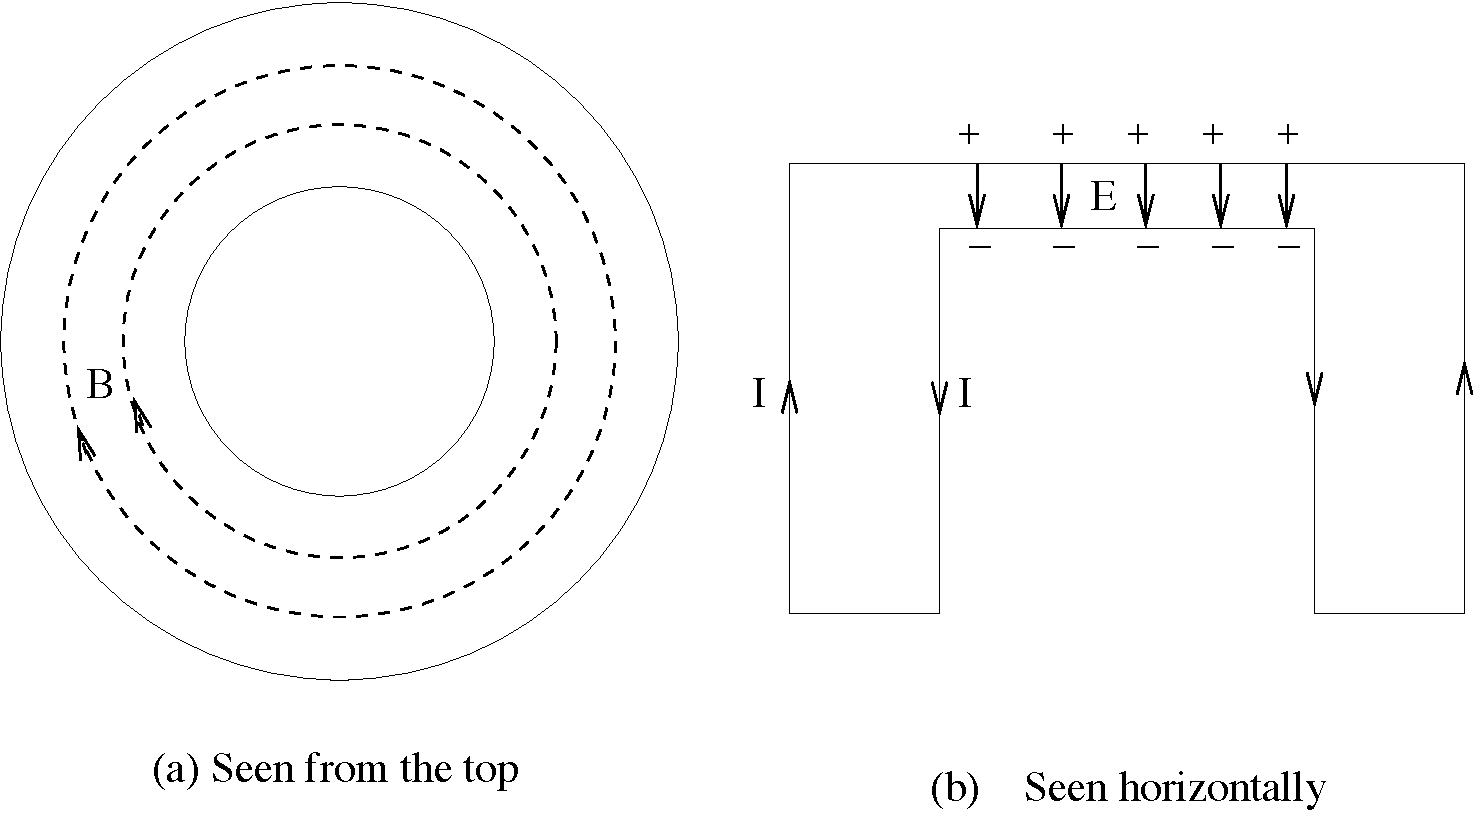
\includegraphics[width = 5cm]{cavity2}
    \caption{The configuration of $\vec{B}$ (a) and $\vec{E}$ field (b).
      The magnetic field lines are circles between the inner and the outer
      cylinders.  The electric field lines are parallel straight lines
      between the top plates.}
    \label{fig:cavity2}
  \end{figure}

\section{Problem \thesection: Purcell 8.9}
\subsection{Problem}
  Using the equations 10 and 13 in Purcell (below), express the effect of
  damping on the frequency of a series $RLC$ circuit.
  \begin{equation*}
    \omega^2 = \frac{1}{LC} - \alpha\frac{R}{L} + \alpha^2 = \frac{1}{LC} - \frac{R^2}{L^2}
  \end{equation*}
  \begin{equation*}
    Q = \omega \frac{\text{energy stored}}{\text{average power dissipated}}
  \end{equation*}
  Let $\omega_0 = 1 / \sqrt{LC}$ be the frequency of the undamped circuit.
  Suppose enough resistance is added to bring $Q$ from $\infty$ down to
  1000.  By what percentage is the frequency $\omega$ thereby shifted from
  $\omega_0$?

  \begin{center}
    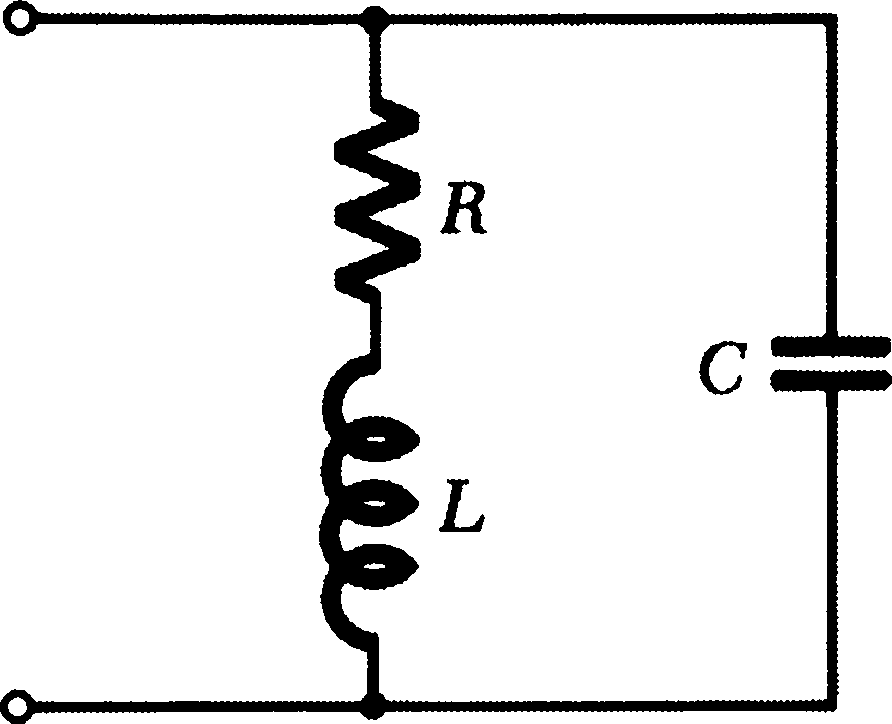
\includegraphics[width = 0.5\textwidth]{figpu809}
  \end{center}
\subsection{Solution}
  Use eqs.(13) or (14) of Purcell p.301-302.
  \begin{equation}
  R=\frac{\omega L}{Q} \quad\to\quad \frac{R}{L}=\frac{\omega}{Q}\,.
  \end{equation}
  Plug this into eq.(10) of Purcell p.299.
  \begin{align}
  \omega^2 & = \omega_0^2-\frac{\omega^2}{4Q^2},\\
  \text{so} \qquad \omega & = \omega_0 \left(1+\frac{1}{4Q^2}\right)^{-1/2}\\
  & = \omega_0\frac{2Q}{\sqrt{1+4Q^2}}.
  \end{align}
  where $\omega_0=1/\sqrt{LC}$.  The percentage change is
  \begin{align}
  \text{Percentage change} & = \frac{\omega_0-\omega}{\omega_0}\times
  100\%\nonumber\\
  & = \left[1-\left(1+\frac{1}{4Q^2}\right)^{-1/2}\right]\times 100\%\nonumber\\
  &\approx & \frac{1}{8Q^2}\times 100\%\nonumber\\
  & = 1.25\times 10^{-5} \%,
  \end{align}
  for $Q=1000$.  (The binomial expansion was used to simplify the exact formula.)

\section{Problem \thesection: Purcell 8.12}
\subsection{Problem}
  Let $V_{AB} = V_B - V_A$, in this circuit.  Show that $|V_{AB}|^2 =
  V_0^2$ for any frequency $\omega$.  Find the frequency for which $V_{AB}$
  is $90^\circ$ out of phase with $V_0$.

  \begin{center}
    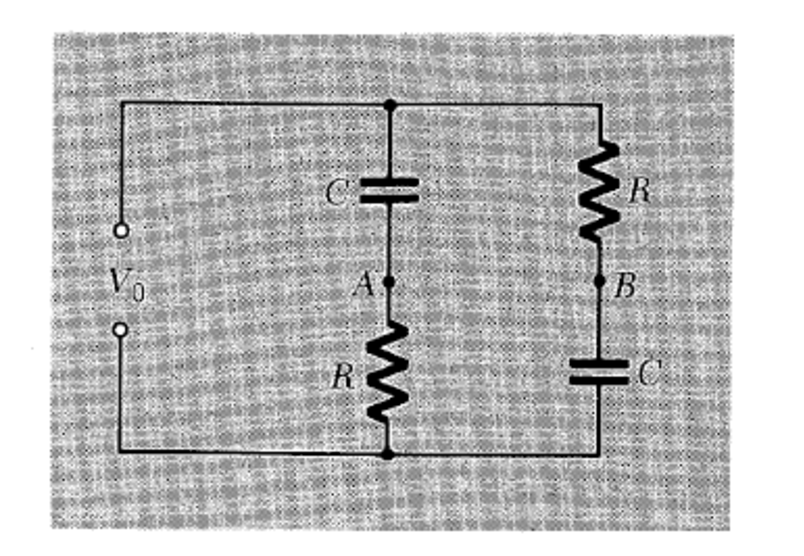
\includegraphics[width = 0.5\textwidth]{figpu812}
  \end{center}
\subsection{Solution}
  \begin{figure}[H]
    \centering
    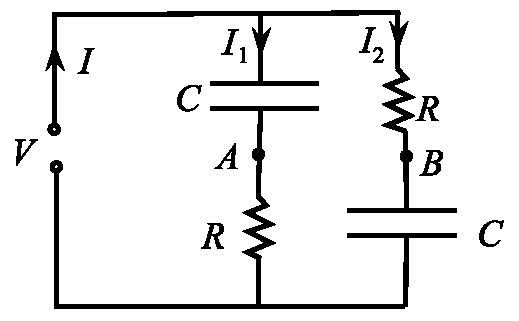
\includegraphics[width = 5cm]{Purcell812}
    \caption{Circuit with resistors and capacitors}
    \label{RCRC}
  \end{figure}
  Considering the two circuit loops that contain $V_0$, we can find
  the following equations relating the currents $I_1$ and $I_2$ to the voltage
  $V_0$:
  $$ V_0 = I_1 Z_1 = I_1\left( (\frac{-i}{\omega C}) + R\right) \qquad V_0 = I_2 Z_2  = I_2\left(R + (\frac{-i}{\omega C})\right)$$
  The voltage $V_{AB} = V_B - V_A$ is then:
  $$V_{AB} = -I_2 R + I_1( \frac{-i}{\omega C})$$
  Substituting for the currents $I_1$ and $I_2$, we find:
  $$V_{AB} = -\frac{V_0 R}{R +( \frac{-i}{\omega C})} + \frac{V_0( \frac{-i}{\omega C})}{R + (\frac{-i}{\omega
  C})} = -V_0\frac{R + \frac{i}{\omega C}}{R - \frac{i}{\omega C}} =
  V_0\frac{1 - i \omega RC}{1 + i \omega RC}$$
  We can take the absolute value of both side to get:
  $$|V_{AB}|^2 = |V_0|^2\left(\frac{1-i\omega RC}{1+i\omega RC}\right)\left(\frac{1+i\omega RC}{1-i\omega
  RC}\right) = |V_0|^2\frac{1 + (RC\omega)^2}{1 + (RC\omega)^2} =
  |V_0|^2$$
  In order for $V_{AB}$ and $V_0$ to be out of phase by $\phi =
  -{\pi}/{2}$, we must have $$V_{AB} = V_0e^{i\phi} =
  V_0e^{-i\frac{\pi}{2}} = -iV_0$$ Therefore ,
  $$\frac{1 - i \omega RC}{1 + i \omega RC} = -i \quad \implies
  \quad \frac{1- (RC\omega)^2}{1+ (RC\omega)^2} -
  i\frac{2RC\omega}{1+ (RC\omega)^2} =-i$$
  Equating the real parts (the imaginary parts give the same result),
  we find:
  $$1-(RC\omega)^2 = 0  \quad \implies \quad \omega =
  \frac{1}{RC}$$

\section{Problem \thesection: Purcell 8.16}
\subsection{Problem}
  \begin{center}
    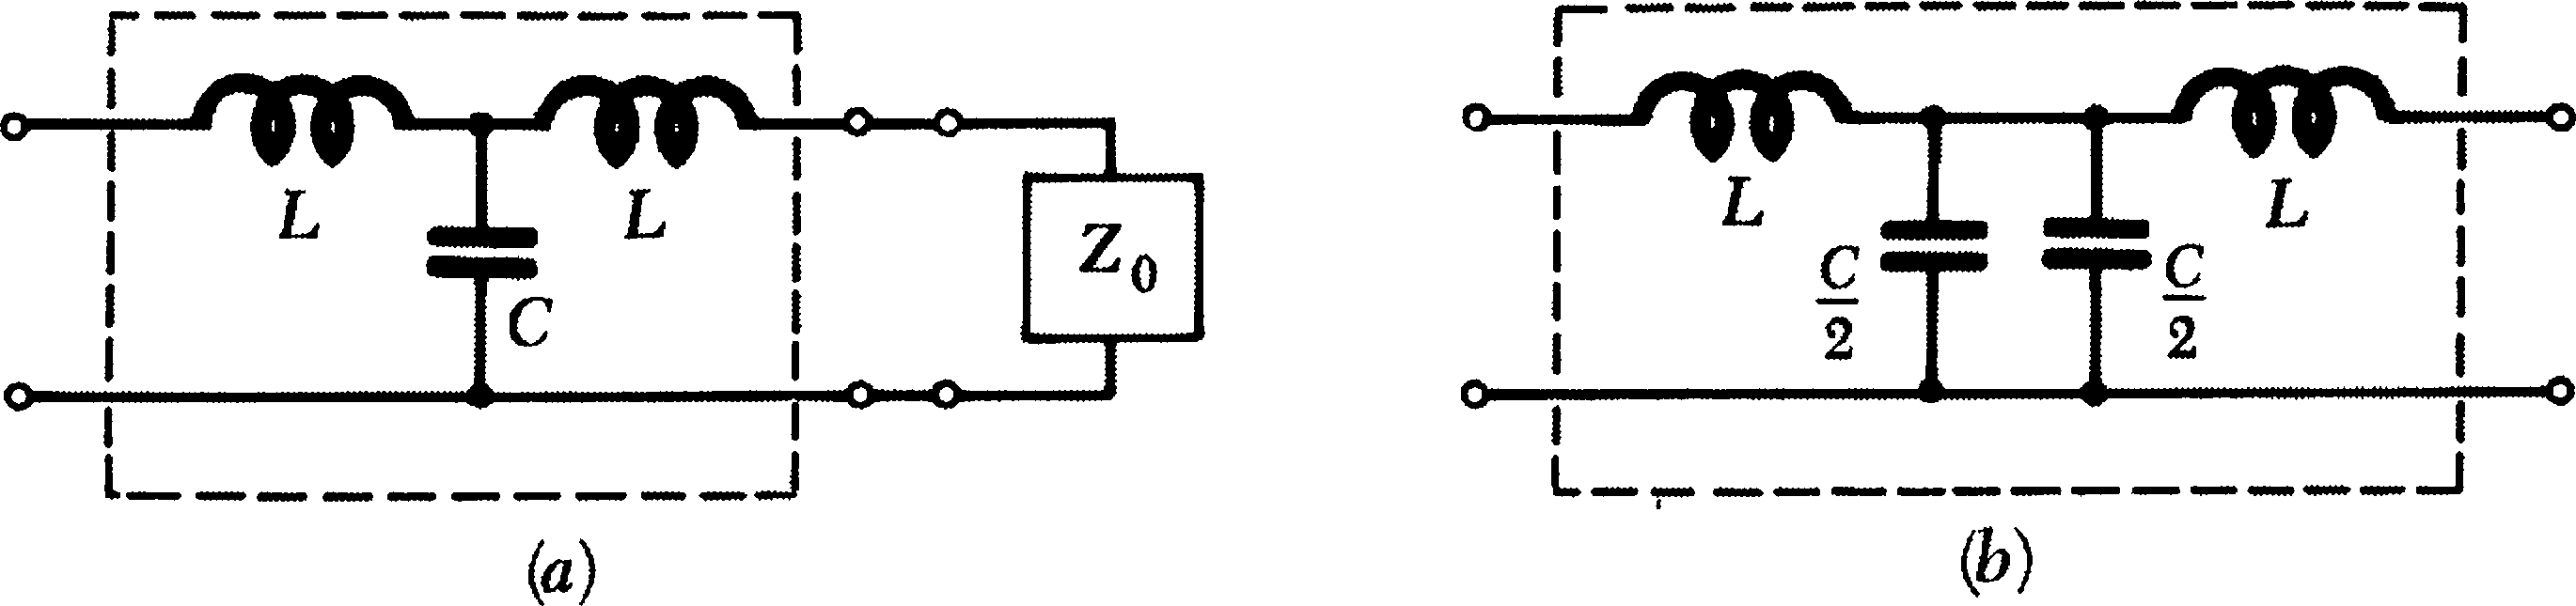
\includegraphics[width = 0.75\textwidth]{pu816}
  \end{center}

  \noindent The box (a) with four terminals contains a capacitor $C$ and
  two inductors of equal inductance $L$ connected as shown.  An impedance
  $Z_0$ is to be connected to the terminals on the right. For a given
  frequency $\omega$ find the value which $Z_0$ must have if the resulting
  impedance across the left terminals is $Z_0$. You will find that the
  required $Z_0$ is a pure resistance $R_0$ provided $\omega^2<2/LC$. What
  is $Z_0$ in the special case $\omega = \sqrt{2/LC}$?  It helps in
  understanding that case to note that the contents of the box (a) can be
  equally well represented by box (b).
\subsection{Solution}
  We combine the impedances like resistances so that the total impedance is
  \[ Z = Z_L + \frac{1}{\frac{1}{Z_C} + \frac{1}{Z_L + Z_0}}\ \ , \]
  with $Z_L = i\omega L$ and $Z_C = 1/i\omega C$. We set this equal to $Z_0$ and simplify to obtain
  \[ Z_0 = \sqrt{-\omega^2L^2 + 2L/C}\ \ .\]
  This will be pure real and thus a pure resistance if
  \[ -\omega^2L^2 + 2\frac{L}{C} >0 \ \ ,\]
  \[ \omega^2 < \frac{2}{LC}\ \ .\]
  In the special case $\omega = \sqrt{2/LC}$, we have $Z_0=0$.
\section{Problem \thesection: Optional Purcell 8.10}
\subsection{Problem}
  Is it possible to find a frequency at which the impedance at the
  terminals of the circuit below will be purely real?

  \begin{center}
    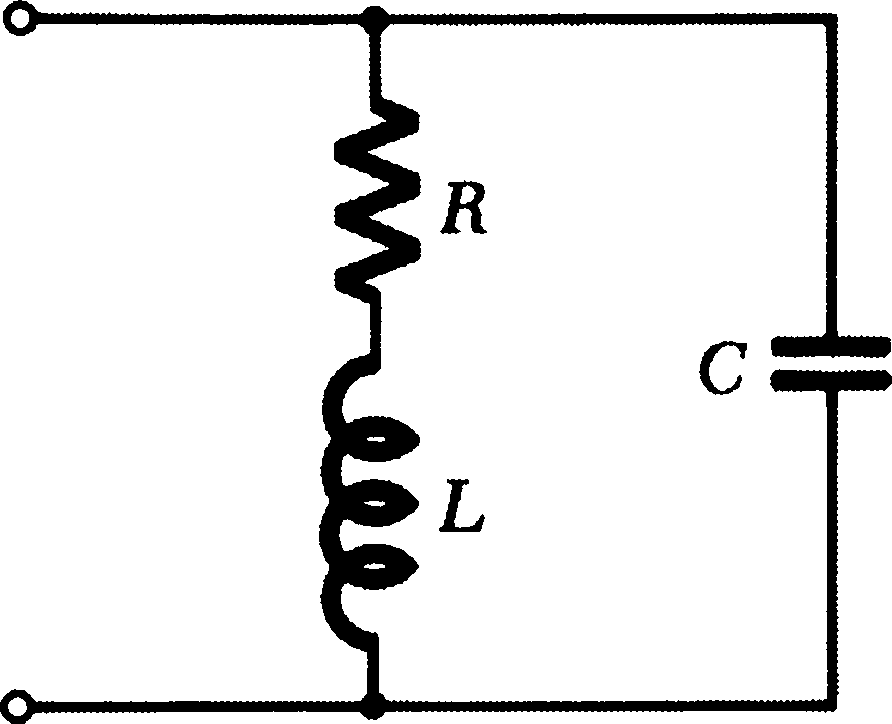
\includegraphics[width = 0.5\textwidth]{figpu810}
  \end{center}
\subsection{Solution}
  \begin{align}
  \frac{1}{Z} & = i\omega C + \frac{1}{R+i\omega L}\nonumber\\
  \frac{1}{Z} & =\left[i\omega C+\frac{R-i\omega L}{R^2+(\omega
  L)^2}\right]\nonumber\\
  & = \left[ i(\omega C-\frac{\omega L}{R^2+(\omega
  L)^2})+(\text{real part})\right].
  \end{align}
  To make $Z$ purely real, $Z^{-1}$ must be real.  So
  \begin{align}
  \omega C & = \frac{\omega L}{R^2+(\omega L)^2},\\
  \omega & = \sqrt{\frac{L-CR^2}{CL^2}}.
  \end{align}

  Note that the argument inside a square root must be positive.
  Therefore the condition under which it is possible to find
  a frequency so that $Z$ is purely real is
  \begin{equation}
  L/C>R^2.
  \end{equation}
\section{Problem \thesection: Optional Purcell 8.13}
\subsection{Problem}
  Show that, if the condition $R_1R_2 = L / C$ is satisfied by the
  components of the circuit below, the difference in voltage between points
  $A$ and $B$ will be zero at any frequency.  Discuss the suitability of
  this circuit as an AC bridge for measurement of an unknown inductance.

  \begin{center}
    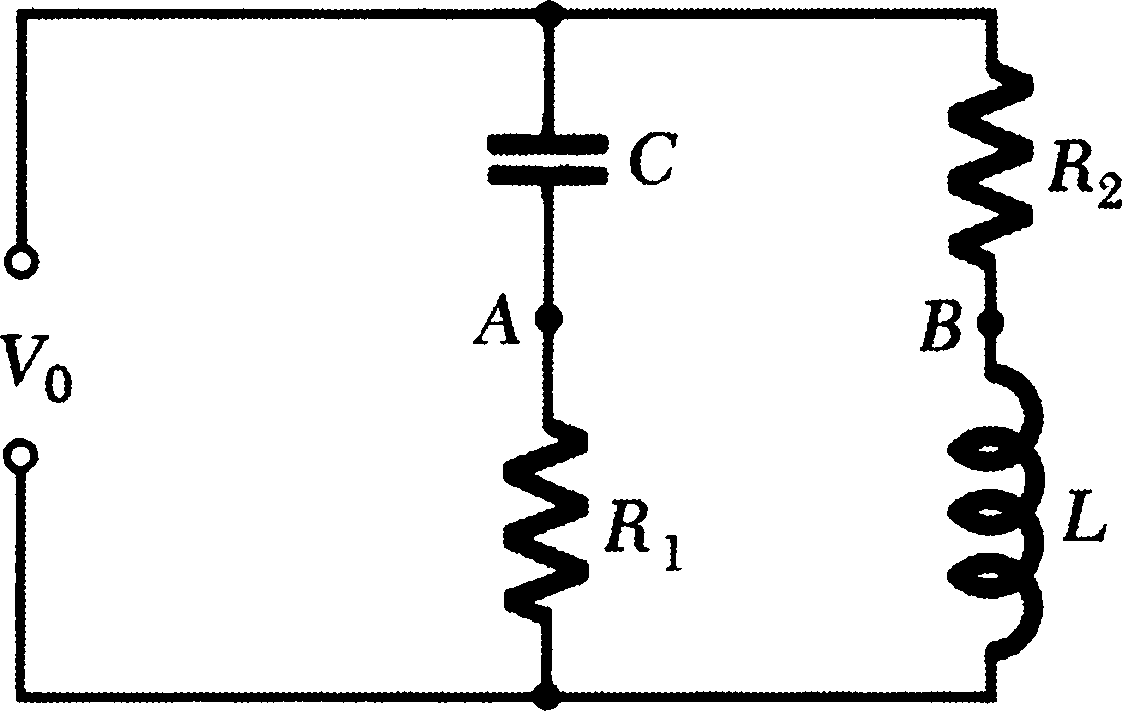
\includegraphics[width = 0.5\textwidth]{figpu813}
  \end{center}
\subsection{Solution}
  Refer to the figure for Problem 8.13 of Purcell p.321.  The impedance
  of the left path ($C-R_1$) and the right ($R_2 - L$) are respectively
  \[Z_1=R_1-\frac{i}{\omega C},\;\;\;\;\;\; Z_2=R_2+i\omega L.\]
  Set the voltage at the bottom of the circuit to be zero.  Then the
  voltages at the points A and B are respectively
  \begin{align}
  V_A & = \frac{V_0}{Z_1} R_1= \frac{V_0 R_1}{R_1-\frac{i}{\omega
  C}},\nonumber\\
  V_B & = \frac{V_0}{Z_2} (i\omega L)=\frac{V_0 i\omega L}{R_2+i\omega L}.
  \end{align}
  Solve $V_A=V_B$.
  \begin{align}
  R_1(R_2+i\omega L) & = i\omega L (R_1-\frac{i}{\omega C})\nonumber\\
  \text{or}\qquad\qquad R_1 R_2 & = L/C.\label{eqn5:condition}
  \end{align}

  Since condition (\ref{eqn5:condition}) doesn't depend on the value of
  frequency, we conclude that, if condition (\ref{eqn5:condition}) is
  satisfied, the voltage difference between points A and B will be zero
  at any frequency.\\

  We may employ this condition to measure unknown inductance.  The
  circuit is exactly the same, but we connect points A and B by an AC
  voltmeter.  The values of $R_1$, $R_2$ and $C$ are known; at least one
  of the resistance should be adjustable.  We then adjust the resistance
  so that the reading in the voltmeter vanishes.  If necessary, we may
  adjust the frequency to check that this vanishing doesn't depend on
  frequency.  At the vanishing point the condition
  (\ref{eqn5:condition}) is satisfied and the inductance is measured by
  $L=R_1 R_2 C$.
\section{Problem \thesection: Optional Purcell 8.14}
\subsection{Problem}
  In the laboratory, you find an inductor of unknown inductance $L$ and
  unknown internal resistance $R$.  Using a DC ohm-meter, an AC volt-meter
  of high impedance, a 1-microfarad capacitor, and a 1000-Hz signal
  generator, determine $L$ and $R$ as follows: According to the ohm-meter,
  $R$ is 35 ohms.  You connect the capacitor in series with the inductor
  and the signal generator.  The voltage across both is 10.1 volts.  The
  voltage across the capacitor alone is 15.5 volts. You note also, as a
  check, that the voltage across the inductor alone is 25.4 volts.  How
  large is $L$?  Is the check consistent?
\subsection{Solution}
  Consider the RLC in series.
  \begin{equation}
  Z_{LR}=R+i\omega L\,,\qquad Z_c=-i/\omega C\,,\qquad
  Z_{\text{total}}=R+i(\omega L-1/\omega C)\,.
  \end{equation}

  From the potential across both and across the capacitor,
  \begin{align}
  \frac{V_{\text{total}}}{V_C}& =\frac{Z_{\text{total}}}{Z_C}=i\omega
  CR+(1-\omega^2 CL)\,,\\
  \text{so}\qquad \left| \frac{V_{\text{total}}}{V_C}\right| & =
  \sqrt{(\omega CR)^2+(1-\omega^2 CL)^2}\,,
  \end{align}

  After doing some math, we find the expression for L,
  \begin{equation}
  \qquad L = \frac{1}{\omega^2 C}\left[
  1\pm \sqrt{\left|\frac{V_{\text{total}}}{V_C}\right|^2-(\omega CR)^2}
  \right]
  \end{equation}

  Plug in $\omega=2\pi f=2\pi\times 1000\text{ Hz}$,
  $V_{\text{total}}=10.1\text{ volts}$, $V_C=15.5\text{ volts}$,
  $C=10^{-6}\text{ farad}$, $R=35\text{ ohm}$, we get
  \[ L= 0.041 \text{ henry}\qquad\text{or}\qquad 0.0098\text{ henry}.\]

  To check the consistency, calculate the ratio
  \begin{align}
  \frac{V_{LR}}{V_C}& =\frac{Z_{LR}}{Z_C}=i\omega CR-\omega^2 CL\\
  \text{so}\qquad \left|\frac{V_{LR}}{V_C}\right| & = \sqrt{(\omega
  CR)^2+(\omega^2 CL)^2}\\
  & = 1.63 \text{ for L=0.041 henry}\nonumber\\
  & & 0.45\text{ for L=0.0098 henry}.
  \end{align}

  The measurement gives $\left|\frac{V_{LR}}{V_C}\right| =
  25.4/15.5=1.64$.  So the correct value for $L$ is $L=0.041$ henry and the
  check is consistent.
\end{document}
